\documentclass[]{article}
\usepackage[a4paper, total={6in, 10in}]{geometry}
\usepackage[utf8]{inputenc}
\usepackage{hyperref}
\usepackage[backend=biber]{biblatex}
\addbibresource{report.bib}
\usepackage{listings}
\usepackage{graphicx}
\usepackage{caption}

\begin{document}

\begin{center}
  {\large Data Mining - ID2222}\\
  \vspace{7mm}
  {\huge Homework 1\\[1ex]}
  {\Large Finding Similar Items: Textually Similar Documents}\\
  \vspace{7mm}  
  {André Silva - Jérémy Navarro\\}
  \vspace{4mm}
  {\large November 9, 2020\\}
\end{center}

\section{Overview}

We chose \textit{Python} as the programming language and an \textsc{OOP} approach for the development of the project.\\
\\
Information about the structure of the project, as well as instructions on how to run it follow:

\begin{lstlisting}[language=bash]
$ unzip homework1.zip
$ cd homework1/
$ python3 main.py
\end{lstlisting}
\\
\\
The project is composed by the following files:

\begin{itemize}
    \item \texttt{testFiles/}: Directory containing example documents and the SMS Spam Collection~\cite{sms}.
    \item \texttt{classes.py}: Contains the classes implementing the several stages of finding textually similar documents.
    \item \texttt{main.py}: The executable script which performs experimentation on the SMS Spam Collection~\cite{sms}, and demonstrates the usage of the classes.
\end{itemize}

\section{Classes}

\subsection{Shingling}

The class \textbf{Shingling} takes 3 arguments:
\begin{itemize}
  \item \texttt{document}: Path of the document or document
  \item \texttt{k}: Size of each shingle
  \item \texttt{isFile}: \texttt{True} if \texttt{document} is a path to a file. Default is \texttt{True}
\end{itemize}
\\
\\
The first step consists in parsing the file's content into a string, if \texttt{document} is a file path.

After this, we compute the shingles of size \textbf{k}, which are put in an ordered set, after being hashed with \textbf{CRC32}~\cite{crc32}. We use this hash function as it allows us to represent each shingle as a 4B integer.

\subsection{CompareSets}
\label{sec:cs}

The class \textbf{CompareSets} takes 2 arguments:
\begin{itemize}
  \item \texttt{set1}: Set of ordered hashed shingles
  \item \texttt{set2}: Set of ordered hashed shingles
\end{itemize}
\\
\\
The class computes the \textbf{Jaccard Similarity} of the two sets. For that, we iterate over the values of \texttt{set1} and check if they are present in \texttt{set2}. We use the result of this computation in the formula of the \textbf{Jaccard Similarity}.

\subsection{MinHashing}

The class \textbf{MinHashing} takes 3 arguments:
\begin{itemize}
    \item \texttt{maxVal}: Maximum value of any hashed shingle. Default value is $2^{32}$
    \item \texttt{k}: Number of hash functions to be generated. Default value is 100
\end{itemize}
\\
\\
We start off by generating the \texttt{k} independent hash functions. To do this, we need to generate \texttt{k} values of \texttt{a}, \texttt{b} and compute \texttt{c}. \texttt{a} and \texttt{b} are random integers with a lower value than \texttt{maxVal}, while \texttt{c} is a prime number slightly higher than \texttt{maxVal}, as to reduce colisions.

With the hash functions generated, we can now compute the minimum hash values for each of them, given a set. The output of this is a document signature.

\subsection{CompareSignatures}

The class \textbf{CompareSignatures} takes 2 arguments:
\begin{itemize}
    \item \texttt{sig1}: Signature of a document
    \item \texttt{sig2}: Signature of a document
\end{itemize}
\\
\\
This class performs a simple task, computing the percentage of elements of the signatures that are equal. This results in an approximation of the \textbf{Jaccard Similarity} computed in ~\ref{sec:cs}.

\subsection{(\textit{Bonus}) LSH}

The class \textbf{LSH} takes 3 arguments:
\begin{itemize}

  \item \textbf{b} Integer of the number of bands
  \item \textbf{r} Integer of the number of rows
  \item \textbf{listMinHash} List of min-hashed signatures
  
\end{itemize}\\
\\
First, we populate each band with the hash values of the corresponding parts of the signatures. The hash function used is the built in hash function for tuples.\\
\\
Then, for every row in the band we check if there are equal hash values in other rows. As we are working with hash values, this is the equivalent of placing them in buckets.\\
\\
The pairs of rows found in this last step represent the pairs of possible candidates.

\section{Results}

In Figure~\ref{fig:1}, we can see partial results of running out experiment. 

We can notice that the number of candidate pairs generated at the end of \textbf{LHR} is very small when compared to the number of possible pairs of documents. 

We can also see that, for the example of pair showed, the estimated similarity using \textbf{MinHash} is close to the \textbf{Jaccard Similarity} of the same documents.

\begin{figure}[h!]
    \centering
    \captionsetup{justification=centering}
    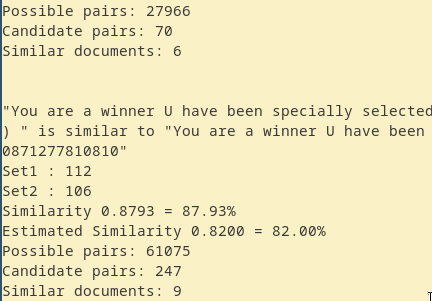
\includegraphics[width=0.4\textwidth,height=\textheight,keepaspectratio]{../results.png}
    \caption{partial results of running \texttt{main.py}.}
    \label{fig:1}
\end{figure}

\pagebreak

In Figure~\ref{fig:2}, the results of our experiment are shown.

We can see that the relation between the size of the dataset and the execution time is, approximately, linear. This means the algorithm scales relatively well as we increase the size of the dataset, something that wouldn't happen if we tried to compute the \textbf{Jaccard Similarity} between all possible pairs of documents.

\begin{figure}[h!]
    \centering
    \captionsetup{justification=centering}
    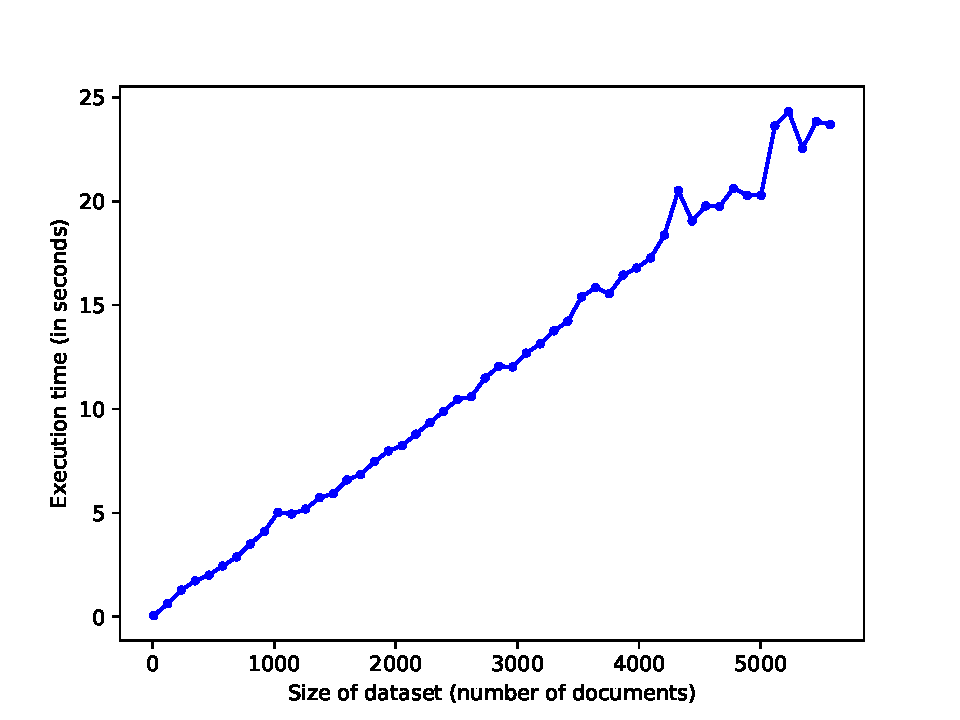
\includegraphics[width=0.4\textwidth,height=\textheight,keepaspectratio]{../datasetsize_execution.pdf}
    \caption{Execution time (in seconds) versus the size of the dataset~\cite{sms}.}
    \label{fig:2}
\end{figure}

\printbibliography

\end{document}
